\chapter{Implementation}\label{ch:implementation}
We implemented \trussFabName{} as a plug-in for the 3D modeling software \textit{SketchUp}. It is primarily written in Ruby and JavaScript.\unsure{Do we assume TrussFormer is a new product, which uses similar functionality as TrussFab, or do we say it is an improvement?}

\section{Architecture}
The software can be divided into four components. The most user-facing one is the TrussFab Designer. It contains the user interface and the construction functionalities. The other components can be seen as extensions to the designer. The \textit{Force Analysis} calculates tension force on the created structure. The tensions forces are calculated using an adapted version of the \textit{MSPhysics}\footnote{https://extensions.sketchup.com/en/content/msphysics} physics engine, which is a Ruby wrapper around the C++ physics engine \textit{NewtonDynamics}\footnote{http://newtondynamics.com/forum/newton.php}.\\
This physics engine is also used by another component, the \textit{Hinge Placement Algorithm}. It uses the physics features to detect changing angles between Edges, indicating the need for a hinge at a Hub.\\
The export function using OpenSCAD will be explained in section \ref{sec:openscad_impl}.
\begin{figure}[!h]
    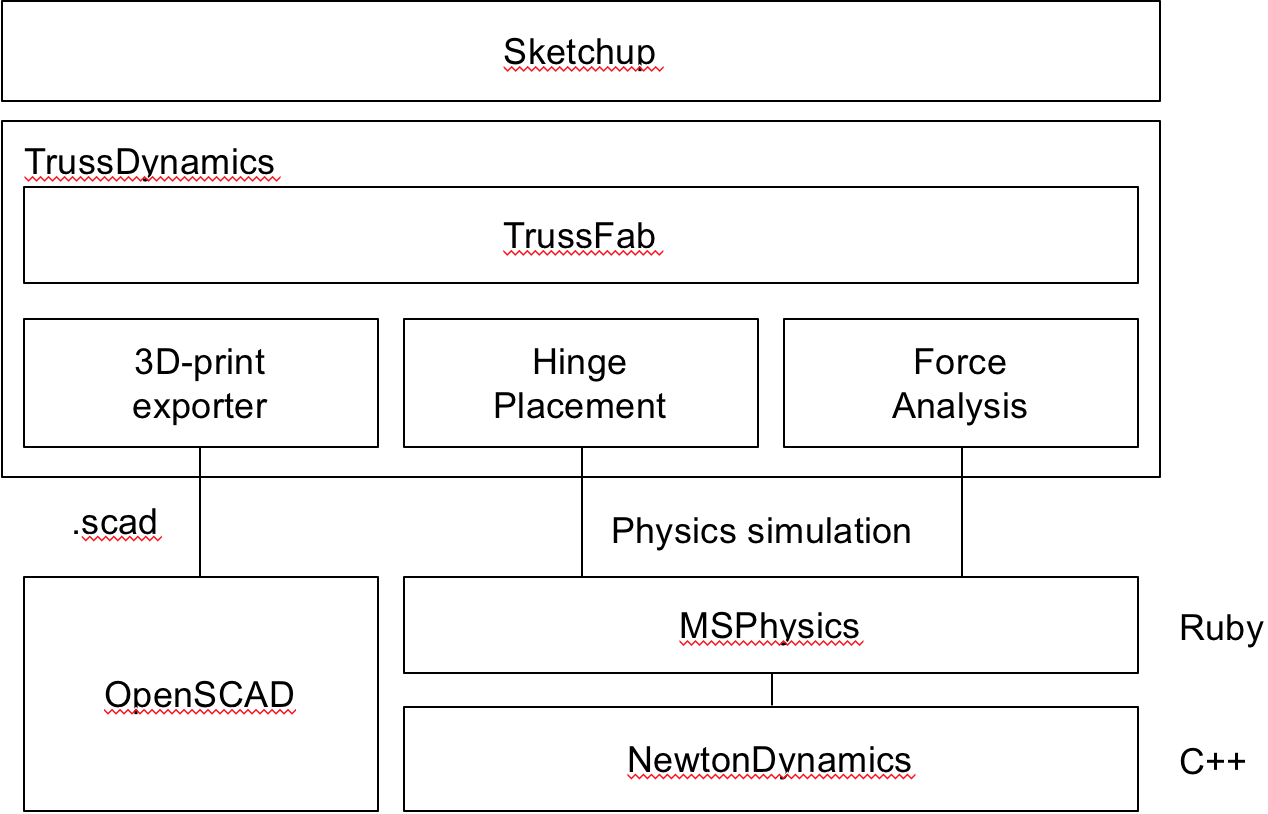
\includegraphics[width=\textwidth]{Implementation/TrussFab_Architecture_Overview.png}
    \centering
    \caption{TrussFab Architecture}
    \label{fig:architecture}
\end{figure}
The structure diagram in figure \ref{fig:architecture} shows an overview of the components. Details for each component will be explained later in this chapter.

\subsection{Designer}
All components are stored in a graph structure. The building parts are \textit{Edges}, \textit{Nodes} and \textit{Triangles}. They all inherit \textit{GraphObject}. The purpose of these objects is providing user-facing functionalities and storing lower-level components. An overview of the graph structure can be seen in \ref{fig:graph}.\\
The \textit{Graph} is implemented as a Singleton \improvement{explain what a Singleton is} that stores and provides access to all GraphObjects, creates new ones and provides convenience functions for user interactions, such as finding the node closest to the mouse cursor. As this class is a singleton, every module of the software has access to the objects.\\
Each of these objects has access to its underlying logic-bearing component, called \textit{SketchupObject}.\improvement{Clarify. Either explain what that means (Hubs, Links, Surfaces) or at least have a forward reference} The access to this functionality is, however, not implemented in this superclass, but in each subclass, having the specific name as an accessor. This design decision was made to improve code readability, and decrease coding errors caused by accessing the wrong SketchupObject.\improvement{Show before and after code snippet}\\
\begin{figure}
    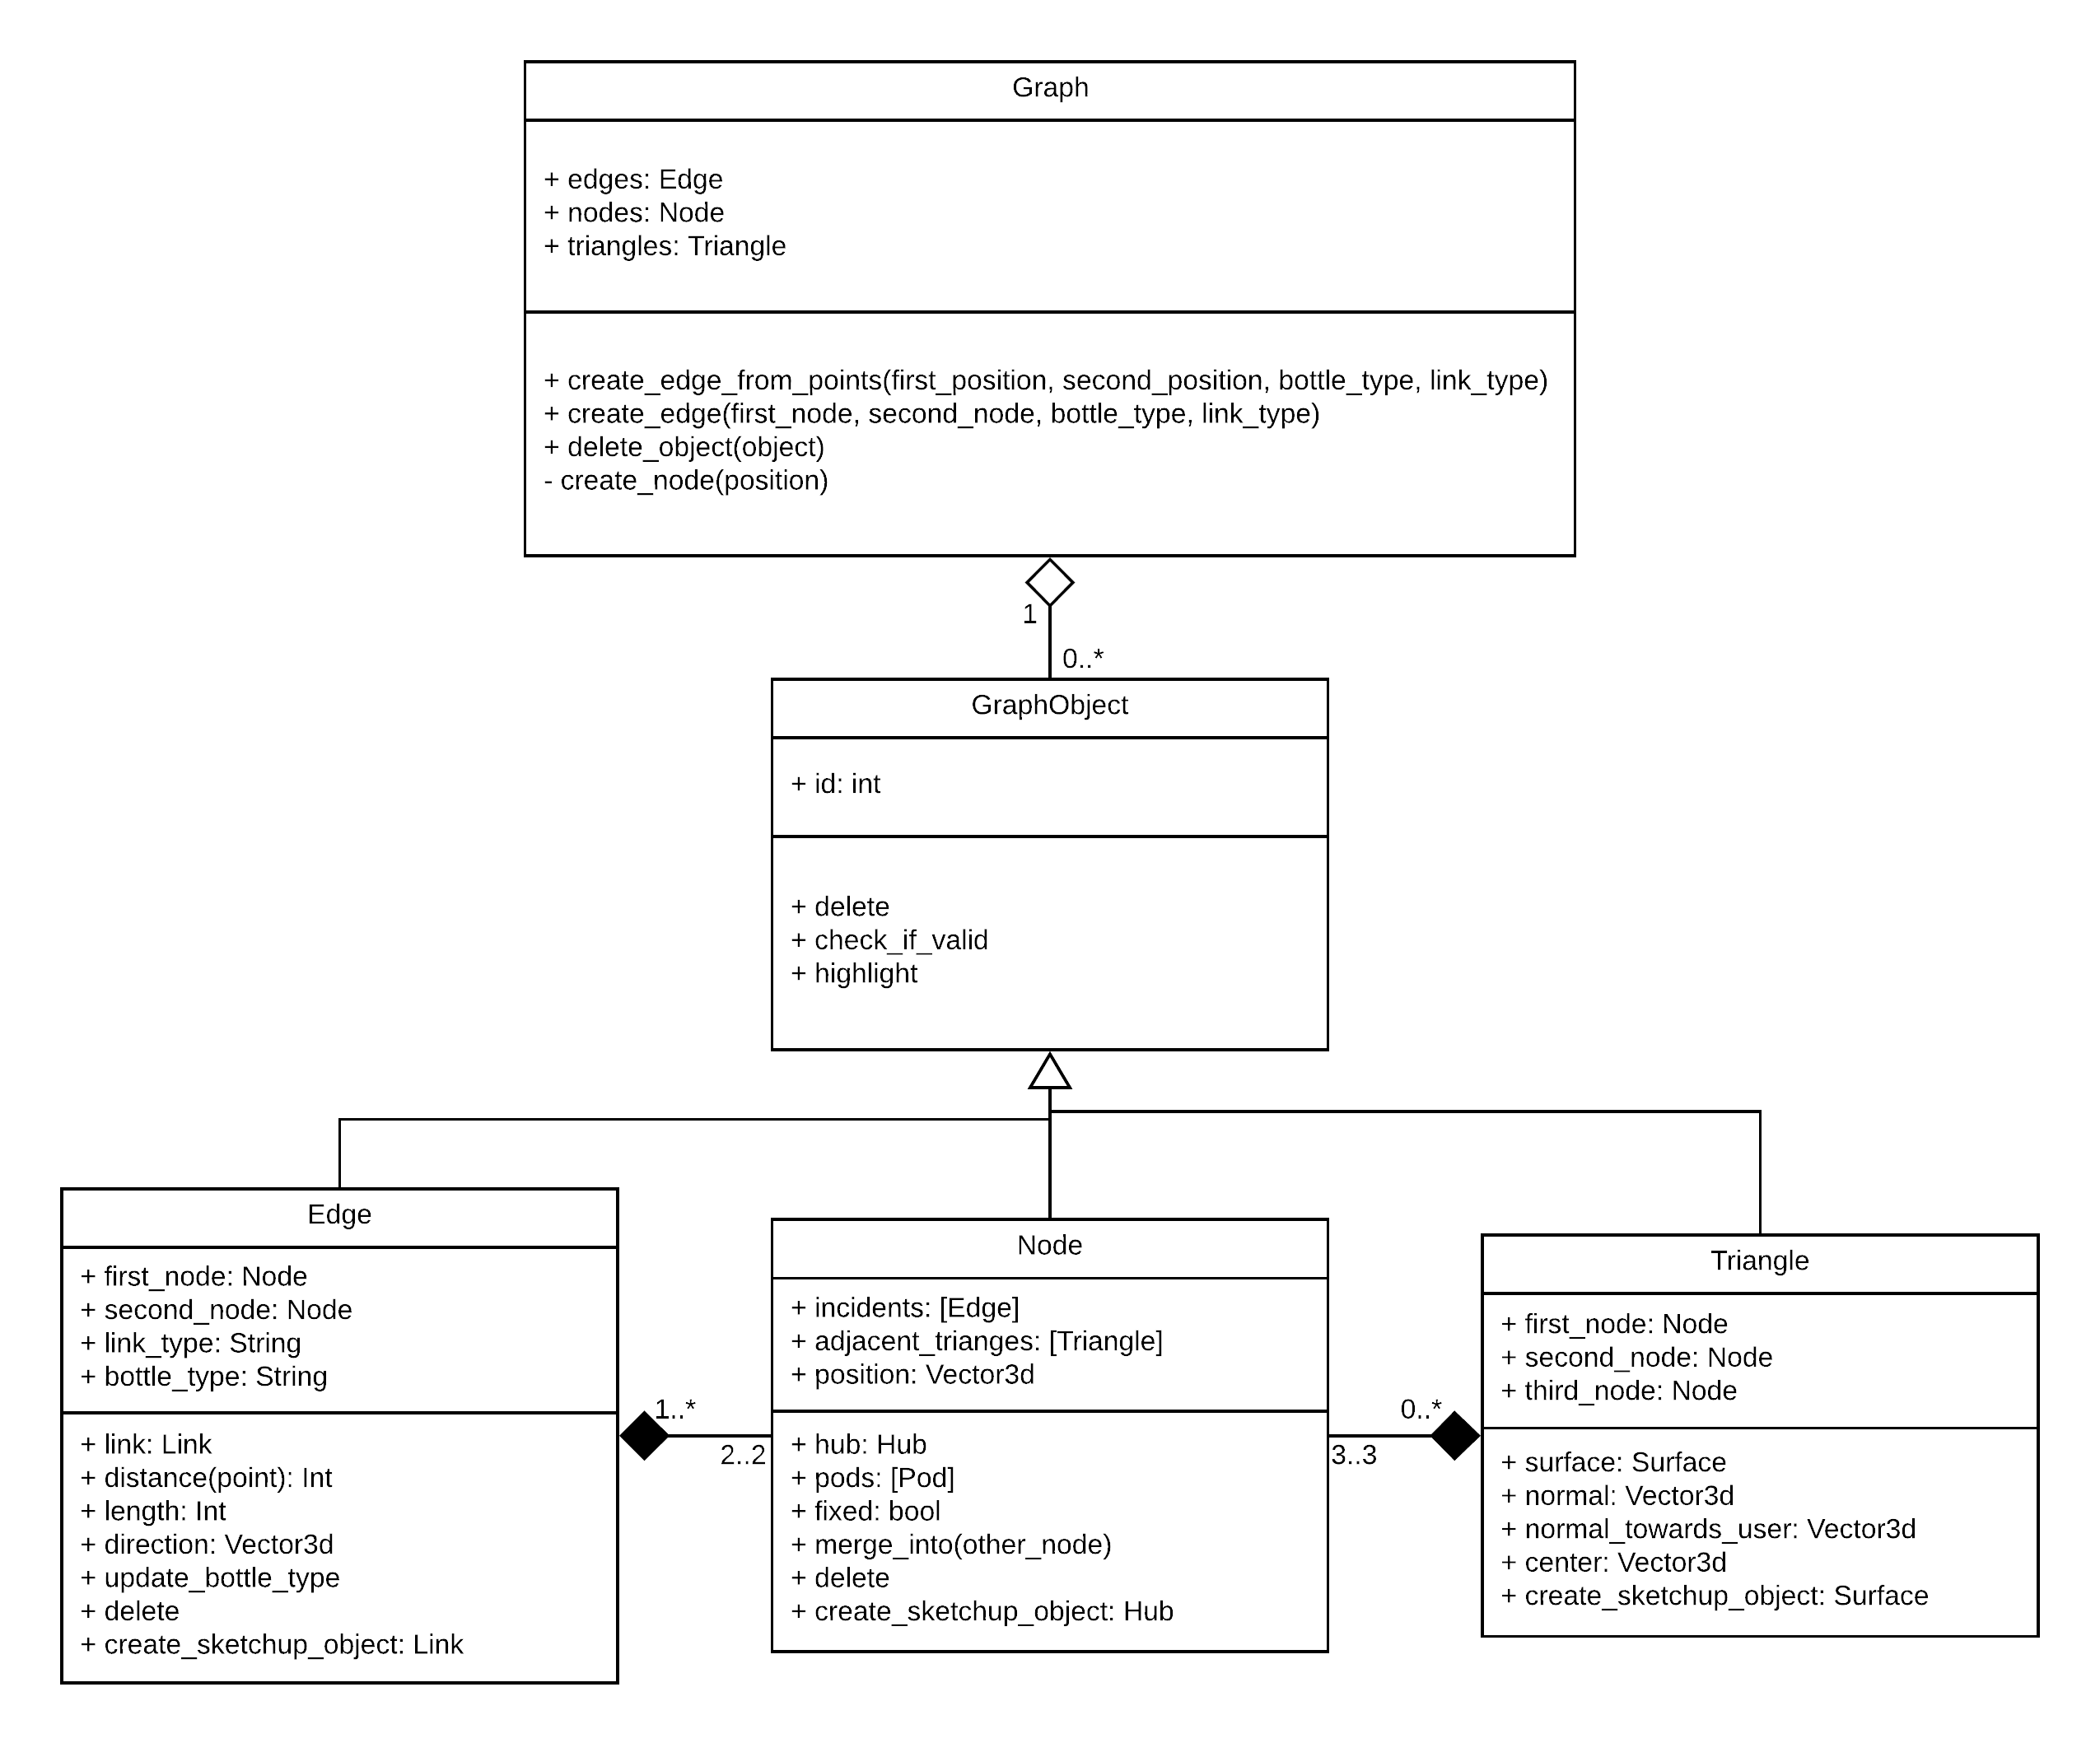
\includegraphics[width=\textwidth]{Implementation/TrussFab_Graph.png}
    \centering
    \caption{Class Diagram showing the high-level Graph Structure of the TrussFab Designer}
    \label{fig:graph}
\end{figure}
The responsibility of the GraphObject class is primarily unifying the way the appearance in SketchUp of the underlying object can be changed as much as possible. This includes highlighting a specific object if the mouse hovers over it, resetting the object to its default state and creating and deleting it. More complex methods need to be implemented in the respective subclass.\\
\textit{Nodes} are the connecting components of the structure. \textit{Edges}, as well as \textit{Triangles} are created based on Nodes. Apart from storing adjacent Edges and Triangles, a Node can specify their positions in the SketchUp world. The Nodes' adjacent objects constantly check if their position has changed and update their SketchUp representation accordingly. If the structure is deformed in such a way that a Node will be at the same position as another one, the Node object can automatically merge into the other Node. The Node will iterate over all its adjacent Edges and tell each one, apart from the Edges that run from the other Node to the Edge the Node is hinging around (i.e. the Edge that is opposite the Node), to exchange itself with the Node it wants to merge into. These Edges are removed from its own adjacent Edges and added to the collection of the new Node. The same happens for all adjacent Triangles. As a last step, the Node deletes itself and all remaining adjacent Edges and Triangles (which will be the Edges and Triangles that got merged). The object will then be adapted according to the new positions using the \textit{Relaxation algorithm}, described in section \ref{sec:relaxation}.\\
\begin{lstlisting}[language=Ruby, label={lst:merging_code}, caption=Merging of two Nodes]
  def merge_into(other_node)
    merged_incidents = []
    @incidents.each do |edge|
      edge_opposite_node = edge.opposite(self)
      next if other_node.edge_to?(edge_opposite_node)
      edge.exchange_node(self, other_node)
      other_node.add_incident(edge)
      merged_incidents << edge
    end
    @incidents -= merged_incidents

    merged_adjacent_triangles = []
    @adjacent_triangles.each do |triangle|
      new_triangle = triangle.nodes - [self] + [other_node]
      next unless Graph.instance.find_triangle(new_triangle).nil?
      triangle.exchange_node(self, other_node)
      other_node.add_adjacent_triangle(triangle)
      merged_adjacent_triangles << triangle
    end
    @adjacent_triangles -= merged_adjacent_triangles

    delete
  end
\end{lstlisting}
Another component that is tightly coupled to Nodes are \textit{Pods}. A Pod acts as a stand for the object and tells TrussFab that this Node should not change its position.\todo{add image}\\
The \textit{Edges} are the most visual components of TrussFab. They are visualized by bottles of different lengths, if they are static links, or as two cylinders forming an actuator, if they can have variable lengths. The Edges handle creating the correct model and changing it if the user decides to place a different kind of Edge. Edges play a big role in the simulation.
The last high-level component in TrussFab is the \textit{Triangle}. A Triangle is primarily used as a convenient access to multiple Nodes or Edges. Most tools that work on Nodes, such as the \textit{Add Weight Tool}, can also be applied to Triangles, adding weight to all three connected Nodes. The Triangle also provides functions for telling the \textit{MouseInput} in where a certain face is directed.\improvement{IMPROVE!}

\subsection{SketchupObjects}
As mentioned before, each GraphObject contains a lower-level \textit{SketchupObject}. These objects are responsible for more complex, lower-level tasks, such as physics calculations, rendering and communication to the simulation engine.\\
Each SketchupObject has a \textit{Sketchup::Entity}, which is a class provided by SketchUp that is capable of handling the representation in SketchUp itself. This includes changing the color of the model, hiding and transforming. On creation, each SketchupObject is also persisted in the entity\todo{find out why exactly I did that}.
\begin{figure}[h!]
    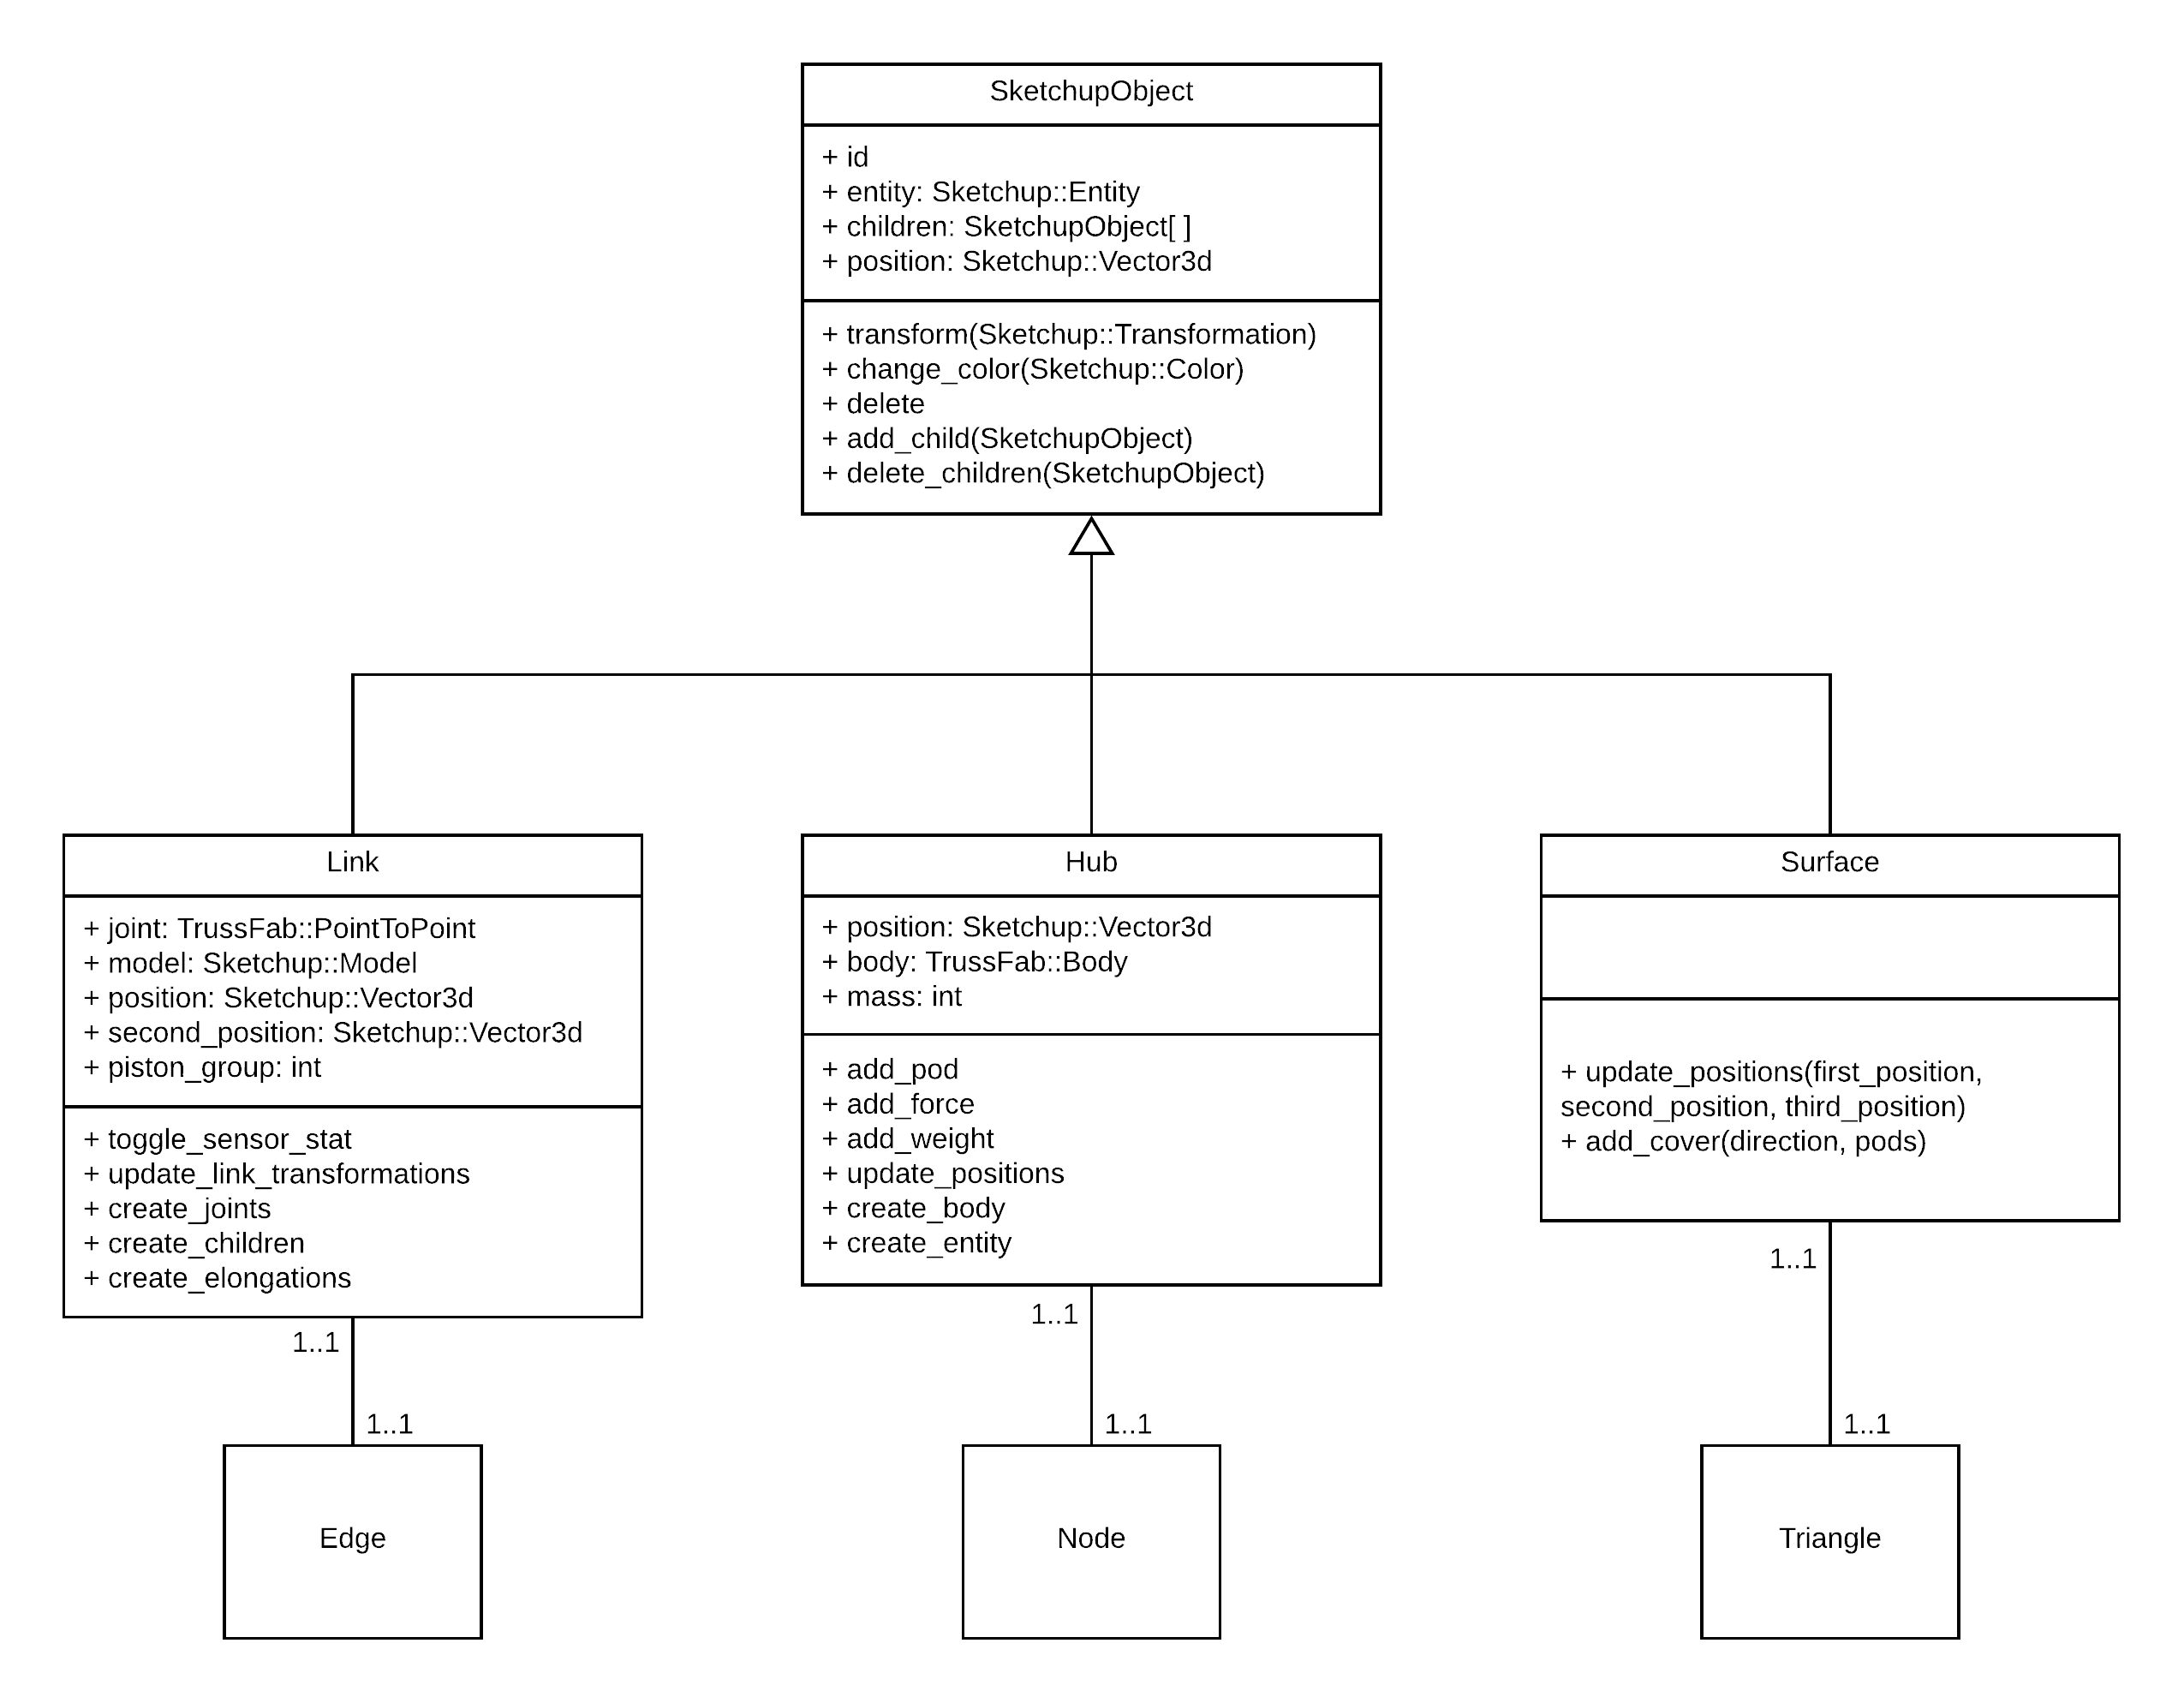
\includegraphics[width=\textwidth]{Implementation/TrussFab_SketchupObjects.png}
    \centering
    \caption{Class Diagram showing the UI components of the graph structure}
    \label{fig:sketchup_objects}
\end{figure}

\subsubsection{Hubs}
\textit{Hubs} are the underlying structures used by Nodes. For ease of calculation and increased performance of the \textit{Simulation} (s.a. section \ref{sec:simulation}), only the Hubs of a structure have physical properties. Hubs therefore have to store information about the object, such as the weight. The weight is calculated based on the number of bottle links and actuators connected to this node. For our system, we measured these values empirically by taking the weight of a screw and half the weight of a bottle link or an actuator per connection and adding it to the average weight of an empty printed hub. The \textit{add weight} and \textit{add force} tools will additionally increase this value, while the Hub also displays the indicators for these tools.\\
These values, together with a few other variables, then form the basis of our simulated structure.

\subsubsection{Links}
\textit{Links} define the connection between two hubs. They are tightly coupled to the physics engine and contain the \textit{Joints}, which are objects used by the engine itself. Available joints are:
\begin{itemize}
    \item TrussFab::PointToPoint - A static connection between two points
    \item TrussFab::PointToPointActuator - A variable-length connection between two points
    \item TrussFab::PointToPointGasSpring - A variable-length connection between two points with a distance-based force factor
    \item TrussFab::GenericPointToPoint - A variable-length connection between two points with a custom force factor
\end{itemize}
The Link is therefore responsible for defining the distance between two Hubs. Because of the nature of truss structures, this can have impact on the whole object and create the variable geometry truss. Joints will be discussed in more detail in the simulation section \ref{sec:simulation}.

\subsubsection{Surface}
The \textit{Surface} is primarily used to visualize what face of the truss the user is currently selecting, by changing the color between three bottles. It can also hold a cover, which has mainly optical purposes, i.e. a user can cover up a surface with a sheet of wood if they want to have this surface closed up after building.

\section{Physics Simulation}\label{sec:simulation}
TrussFabs' force analysis used to be based on \textit{Finite Element Analysis}, calculated asynchronously on a remote server. This provided fairly accurate results and did not require a powerful computer to run. However, TrussFabs' responsibilities evolved during the course of its life and we decided to implement a real-time physics engine inside of our plug-in.\\
We decided to use the SketchUp plug-in \textit{MSPhysics} by Anton Synytsia\footnote{https://github.com/AntonSynytsia/}. MSPhysics is capable of calculating real-time physics on SketchUp elements and creates a customizable physics world in the modeling software. This MSPhysics world has parameters, like gravity, update timestep, and solver model which we can adapt to maximize accuracy and speed of the simulation.\\
The simulation uses the animation feature of SketchUp. A ruby class can act as a Sketchup::Animation when it implements the \textit{nextFrame} method, which must return true until the animation ends. This method is called every time SketchUp receives the signal that a new frame should be rendered. We do that by calling \textit{view.show\_frame} (s.a. listing \ref{lst:simulation}), which will trigger SketchUp to start rendering the next frame based on the simulation updates that happened earlier. We call this function as the first step in our nextFrame method, because this way, SketchUp can start rendering, while our simulation does the next physics update.\\
\begin{lstlisting}[language=Ruby, label={lst:simulation}, caption=Simulation nextFrame method]
def nextFrame(view)
    view.show_frame
    return @running unless @running && !@paused

    update_world
    update_hub_addons
    update_entities

    if (@frame % 5).zero?
      send_sensor_data_to_dialog
    end

    @frame += 1
    update_status_text

    @running
end
\end{lstlisting}
During this update, the physics engine calculates new forces on each physics component of the built object. For that, first all static forces are applied to the object. These are forces added by the \textit{Add Force Tool} or static forces calculated by the \textit{GenericPointToPoint} joints. Using these values and all other intrinsic parameters included in the physics objects, we call the entry point to our MSPhysics plug-in. The \textit{@world.advance} function calculates the change of forces and positions from one timestep to another. In our physics world, one timestep correlates to 1/60s, to achieve realistically timed results assuming that SketchUp itself runs with 60 frames per second.\\
After each world update, the tensions on each link are recorded for visualizing them later. This has to be done, because there could potentially be multiple world updates per render step and we do not want to miss crucial forces.\\
These steps in \textit{update\_world} are done for a specified number of times. In regular animation mode, one world update is calculated per frame, however some tools use the simulation in the background for static checks or other calculations. These tools do not need to display the in-between steps, so they can calculate multiple world updates back-to-back.\\
With the knowledge of the new physics calculations, we can send information about the stress level of each joint to SketchUp. We color the links depending on the tension force on them. A blue color means negative tension force, i.e. pulling force, while red color means positive force, i.e. compressing force. The higher the force, the deeper the color gets.\\
\begin{figure}[h!]
    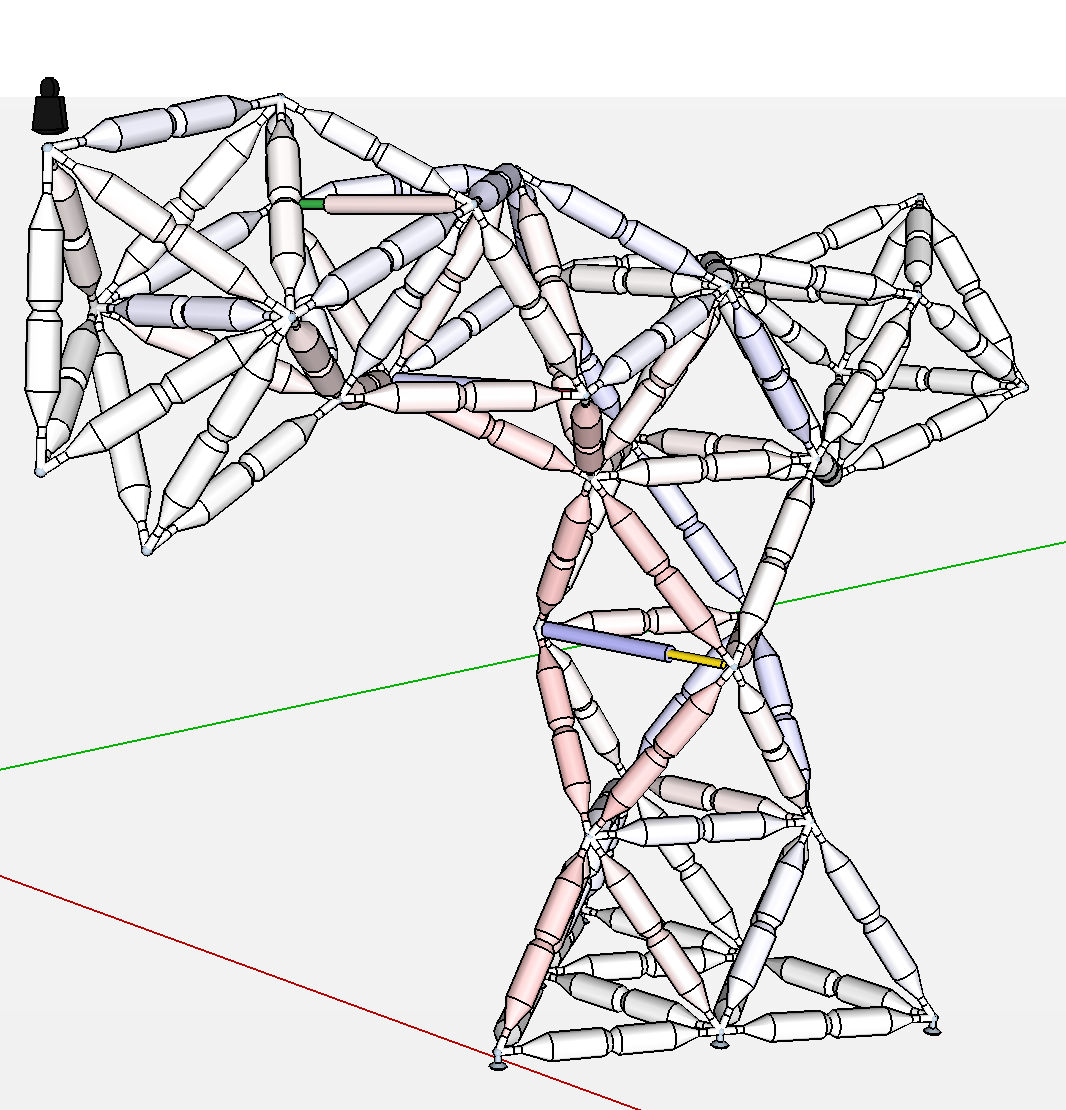
\includegraphics[width=\textwidth]{Implementation/Forces.png}
    \centering
    \caption{Visualization of forces acting on edges. Blue - tension force, red - compression force, white - little or no force}
    \label{fig:force_visualization}
\end{figure}
Once the physics portion of the rendering step is done, our own graph structure has to be updated. For that, each edge and node updates their own positions and transformations based on their internal physics objects.\\
As a last step, sensor data is send to the respective UIs in order to draw a chart depicting physical data.
\section{Minimization Logic}
- elongates and shortens edges so that maximum movement is possible with minimum material use\\
- uses iterative relaxation algorithm, will be explained in \ref{sec:relaxation}

\section{Export}

\section{TrussFab Designer}
The TrussFab Designer provides static sketching functionalities. It can create and display different predefined models, has knowledge about the connections of different components and can modify the resulting objects structure.

\subsection{User Interface}
The user interface (UI) is written in JavaScript. It uses SketchUps' built-in \textit{HtmlDialog} class, which lets us interact with HTML dialog boxes using the Ruby API\footnote{Application Programming Interface}. The HtmlDialog is a modified version of Googles' Chrome browser and supports modern HTML5 code, as well as state-of-the art JavaScript functionalities and extensions.\\
Our user interface has four distinct modules:
\begin{itemize}
    \item the sidebar
    \item the animation pane
    \item force charts
    \item context menus
\end{itemize}

Each of these modules consists of a number of HTML and JavaScript files, which implement the design and functionality of the UI elements, and one Ruby file. The Ruby file is a proxy that communicates between the JavaScript side and the rest of the system. It subscribes to JavaScript callbacks, to react to UI interactions and can directly execute JavaScript code to pass data from ruby to the UI elements.
\begin{lstlisting}[language=Ruby, label={lst:ui_proxy}, caption=excerpt from UI callbacks]
Class AnimationPane
  def add_piston(id)
    @dialog.execute_script("addPiston(#{id})")
  end

  def stop_simulation
    @dialog.execute_script('resetUI();')
  end

  def register_callbacks
    @dialog.add_action_callback('start_simulation') do |_ctx|
      if @simulation_tool.simulation.nil? ||
         @simulation_tool.simulation.stopped?
        start_simulation_setup_scripts
      end
    end

    @dialog.add_action_callback('stop_simulation') do |_ctx|
      unless @simulation_tool.simulation.nil? ||
             stop_simulation
        Sketchup.active_model.select_tool(nil)
      end
    end

    ...
  end
end
\end{lstlisting}

As can be seen in listing \ref{lst:ui_proxy}, these proxy classes have two ways of communicating between Ruby and JavaScript. The \textit{execute\_script} function on the HtmlDialog can call arbitrary code on the UI element at any time. It is possible to pass ruby primitives, such as strings, integers or arrays, through this function call. This makes it possible to a) have complex interactions with the user interface and b) keep state on the ruby side and focus on visualization in JavaScript.\\
The other way works equally asynchronously. JavaScript can send signals to SketchUp. The SketchUp side can register to those callbacks and execute ruby code.

\subsection{Structure Creation}
Terminology:\\
\begin{enumerate}
    \item Edge:
    \begin{enumerate}
        \item Connects two nodes
        \item Can be:
        \begin{enumerate}
            \item Bottle Link
            \item Actuator
            \item PID link
        \end{enumerate}
    \end{enumerate}
\end{enumerate}

\subsection{Modifying the Structure}

\subsection{Relaxation Algorithm}\label{sec:relaxation}

\subsection{OpenSCAD Export}\label{sec:openscad_impl}

\section{TrussFormer Physics Engine}

\subsection{Automatic Actuator Placement (if it works soon-ish)}

\section{Force Control}

\subsection{PID}
